% NeurIPS 2026 poster -- main conference size: 140 cm (W) x 90 cm (H), landscape.
% Build:  latexmk -pdf poster.tex      (two pdflatex passes; images come from make_assets.py)
\documentclass{article}
\usepackage[paperwidth=140cm,paperheight=90cm,margin=0cm]{geometry}
\usepackage[T1]{fontenc}
\usepackage[utf8]{inputenc}
\usepackage[sfdefault,lining,tabular]{FiraSans}
\usepackage{amsmath}
\usepackage{mathtools}
\usepackage{newtxsf}
\usepackage{graphicx}
\usepackage{xcolor}
\usepackage{tikz}
\usetikzlibrary{calc,arrows.meta,positioning}
\usepackage{booktabs}
\usepackage{array}
\usepackage{enumitem}
\usepackage{qrcode}
\usepackage{microtype}

\pagestyle{empty}
\setlength{\parindent}{0pt}

% ---------------------------------------------------------------- colours
% KAIST brand colours (kaist.ac.kr, "Logo Color"):
%   KAIST Dark Blue  PANTONE 286 C   RGB 0/65/145    -- the blue of the KAIST logo
%   KAIST Blue       PANTONE 2925 C  RGB 20/135/200
%   KAIST Light Blue PANTONE 2985 C  RGB 95/190/235
\definecolor{main}{RGB}{0,65,145}
\definecolor{accent}{RGB}{20,135,200}
\definecolor{accentlight}{RGB}{95,190,235}
\definecolor{ink}{HTML}{1A1A22}
\definecolor{muted}{HTML}{55555F}
\definecolor{paper}{HTML}{F8FAFC}
\definecolor{tint}{HTML}{E6EFF9}
% The two ends of the Viridis colormap, for drawings that mimic the heatmaps.
\definecolor{hmlo}{HTML}{440154}
\definecolor{hmhi}{HTML}{FDE725}

% ---------------------------------------------------------------- type scale
\makeatletter
\renewcommand{\normalsize}{\@setfontsize\normalsize{27pt}{36pt}%
  \abovedisplayskip=3.5mm \belowdisplayskip=3.5mm
  \abovedisplayshortskip=2mm \belowdisplayshortskip=3.5mm}
\renewcommand{\small}{\@setfontsize\small{22pt}{28pt}}
\renewcommand{\footnotesize}{\@setfontsize\footnotesize{19.5pt}{24pt}}
\renewcommand{\large}{\@setfontsize\large{32pt}{39pt}}
\renewcommand{\Large}{\@setfontsize\Large{46pt}{52pt}}
\makeatother
\normalsize

\setlist[itemize]{leftmargin=1.1em,itemsep=1.5mm,topsep=1.5mm,parsep=0pt,label={\color{accent}\textbullet}}
\setlist[enumerate]{leftmargin=1.5em,labelsep=0.6em,itemsep=1.5mm,topsep=1.5mm,parsep=0pt,
  label={\bfseries\color{accent}\arabic*}}

% Ragged right without hyphenation: lines break only between words.
\newcommand{\rr}{\raggedright\hyphenpenalty=10000 \exhyphenpenalty=10000 \emergencystretch=3em}

% ---------------------------------------------------------------- building blocks
% \sect{kicker}{title}: a section heading.
\newcommand{\sect}[2]{%
  {\small\bfseries\color{accent}\MakeUppercase{#1}\par}\vspace{1.5mm}%
  {\Large\bfseries\color{main}#2\par}\vspace{3mm}%
  {\color{main}\rule{\linewidth}{1.1mm}\par}\vspace{6mm}}
% \sectx{kicker}{title}{note}: the same, with a note set flush right on the kicker line.
\newcommand{\sectx}[3]{%
  {\small{\bfseries\color{accent}\MakeUppercase{#1}}\hfill{\color{muted}#3}\par}\vspace{1.5mm}%
  {\Large\bfseries\color{main}#2\par}\vspace{3mm}%
  {\color{main}\rule{\linewidth}{1.1mm}\par}\vspace{6mm}}
\newcommand{\sub}[1]{{\large\bfseries\color{ink}#1\par}\vspace{2mm}}
\newcommand{\src}[1]{{\small\color{muted}#1}}
\newcommand{\hl}[1]{\textbf{\color{main}#1}}

% \hmap{width}{file}{caption}: one heatmap with a thin frame and a caption.
\newcommand{\hmap}[3]{%
  \begin{minipage}[t]{#1}\centering\vspace{0pt}%
    \setlength{\fboxsep}{0pt}\setlength{\fboxrule}{0.5mm}%
    \fcolorbox{ink}{white}{\includegraphics[width=\dimexpr\linewidth-1mm\relax]{img/#2.png}}\\[1.5mm]
    {\small\color{ink}#3\par}
  \end{minipage}}

\newcommand{\Wk}{W_{\!k}}
\newcommand{\E}{\mathbb{E}}

\newsavebox{\colA}\newsavebox{\colB}\newsavebox{\colC}\newsavebox{\colD}
\newsavebox{\thmA}\newsavebox{\thmB}\newsavebox{\thmC}\newsavebox{\thmIntro}
\newcommand{\report}[2]{\typeout{POSTER-HEIGHT #1: \the\dimexpr\ht#2+\dp#2\relax}}
% The four columns are set to this fixed height; an overflow shows up in the
% log as `Overfull \vbox'.  \gap{x} is a vertical space that also takes up a
% share of the spare height, so that the columns end on one line.
\newcommand{\colheight}{59.6cm}
\newcommand{\gap}[1]{\vspace{#1 plus 1fill}}
% \dline{math}: a centred formula line, for use directly below a heading.
\newcommand{\dline}[1]{{\centering$\displaystyle #1$\par}\vspace{3mm}}

\begin{document}
\color{ink}

% ======================================================================
% Column A -- background and problems
% ======================================================================
\begin{lrbox}{\colA}\begin{minipage}[t][\colheight][s]{25.2cm}\rr
\sect{Background}{Graphons: limits of dense graphs}

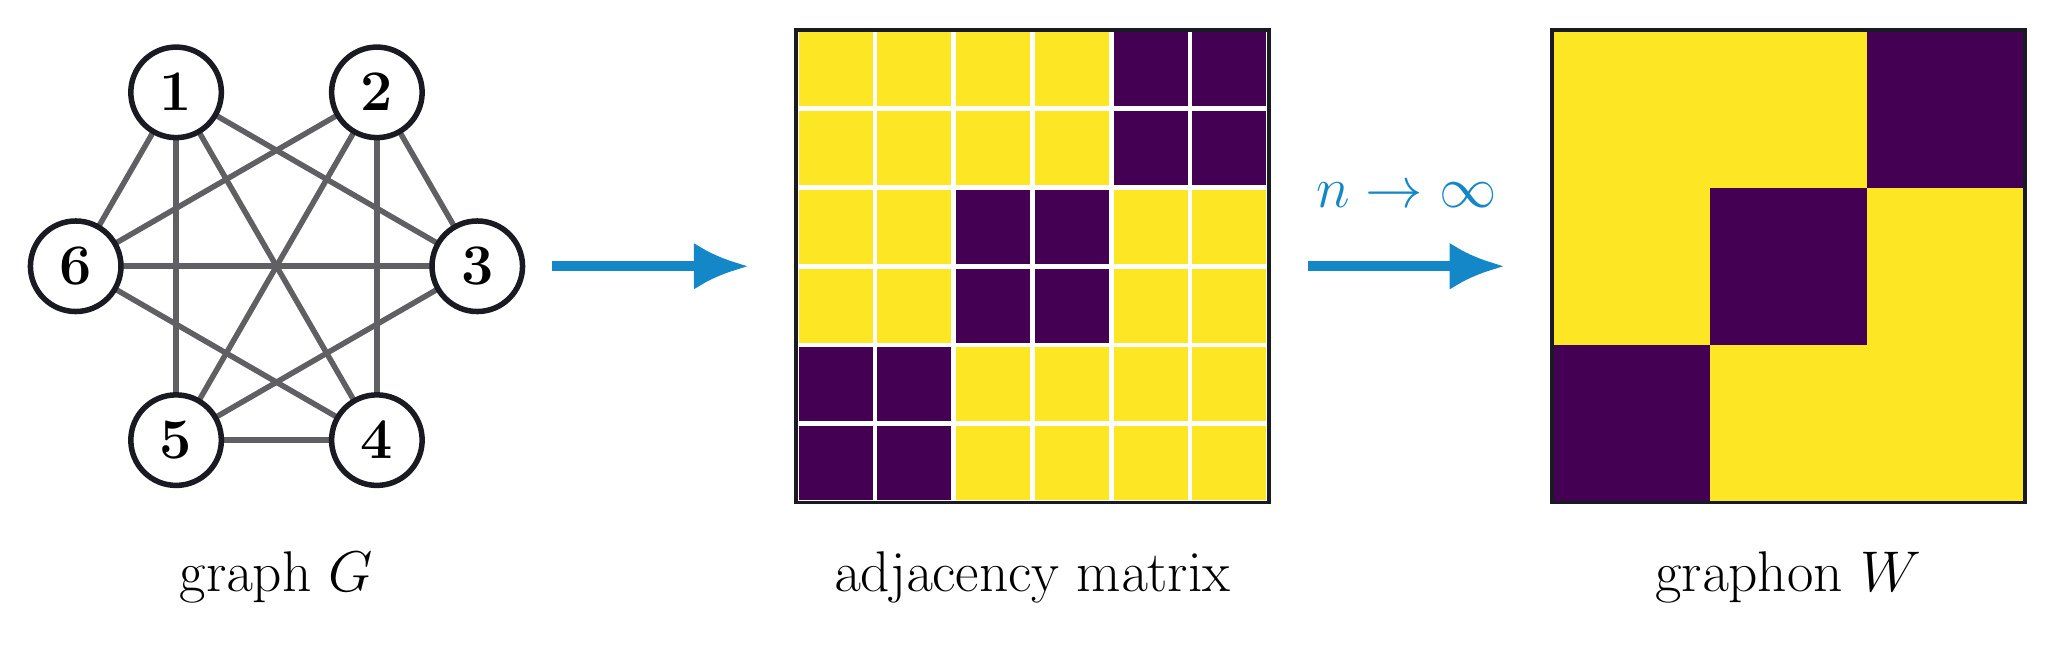
\begin{tikzpicture}[x=1cm,y=1cm]
  % --- a graph: K_{2,2,2}
  \begin{scope}[shift={(3,3)}]
    \foreach \i/\a in {1/120,2/60,3/0,4/-60,5/-120,6/180} \coordinate (n\i) at (\a:2.55);
    \foreach \u/\v in {1/3,1/4,1/5,1/6,2/3,2/4,2/5,2/6,3/5,3/6,4/5,4/6}
      \draw[line width=0.7mm,color=ink!70] (n\u) -- (n\v);
    \foreach \i in {1,...,6}
      \node[circle,draw=ink,line width=0.7mm,fill=white,inner sep=0pt,minimum size=1.15cm]
        at (n\i) {\footnotesize\bfseries \i};
  \end{scope}
  % --- its adjacency matrix (origin bottom-left, as in the heatmaps)
  \begin{scope}[shift={(9.6,0)}]
    \foreach \i in {0,...,5} \foreach \j in {0,...,5} {
      \pgfmathtruncatemacro{\pi}{\i/2}\pgfmathtruncatemacro{\pj}{\j/2}
      \ifnum\pi=\pj \fill[hmlo] (\i,\j) rectangle ++(1,1);
      \else \fill[hmhi] (\i,\j) rectangle ++(1,1);\fi}
    \draw[step=1,white,line width=0.6mm] (0,0) grid (6,6);
    \draw[ink,line width=0.5mm] (0,0) rectangle (6,6);
  \end{scope}
  % --- the limit graphon
  \begin{scope}[shift={(19.2,0)}]
    \fill[hmhi] (0,0) rectangle (6,6);
    \foreach \k in {0,2,4} \fill[hmlo] (\k,\k) rectangle ++(2,2);
    \draw[ink,line width=0.5mm] (0,0) rectangle (6,6);
  \end{scope}
  \draw[-{Latex[length=7mm,width=6mm]},line width=1.3mm,color=accent] (6.5,3) -- (9.0,3);
  \draw[-{Latex[length=7mm,width=6mm]},line width=1.3mm,color=accent] (16.1,3) -- (18.6,3);
  \node[font=\small\bfseries,color=accent] at (17.35,3.9) {$n\to\infty$};
  \node[font=\small,anchor=north] at (3,-0.35) {graph $G$};
  \node[font=\small,anchor=north] at (12.6,-0.35) {adjacency matrix};
  \node[font=\small,anchor=north] at (22.2,-0.35) {graphon $W$};
\end{tikzpicture}

\vspace{5mm}
A \hl{graphon} is a symmetric measurable function $W\colon[0,1]^2\to[0,1]$: the
adjacency matrix of a graph on a continuum of vertices. Dense graph sequences
converge to graphons, and so do the densities of every pattern graph $H$:
\[
  t(H,W)\;=\;\E_{x_1,\dots,x_{v(H)}\sim \mathrm{U}[0,1]}
  \Bigl[\,\prod_{\{i,j\}\in E(H)} W(x_i,x_j)\Bigr].
\]
$t(K_2,W)$ is the edge density, $t(K_3,W)$ the triangle density.

\gap{10mm}
\sect{Problems}{Two variational problems}

\sub{(P1)\; Extremal graph theory}
\vspace{2mm}
\dline{\min_{W}\; t(H,W)\quad\text{subject to}\quad t(K_2,W)=p}
How few copies of $H$ can a graph of edge density $p$ contain? Solved for
cliques only; for $C_5$ only at $p=1-1/k$.
\src{[Razborov 2008; Reiher 2016; Bennett et al.\ 2020]}

\gap{7mm}
\sub{(P2)\; Large deviations of $G(n,q)$}
\vspace{2mm}
\dline{\min_{W}\; h_q(W)\quad\text{subject to}\quad t(H,W)=r^{e(H)}}
\dline{h_q(W)=\int_{[0,1]^2}\mathrm{KL}\bigl(\mathrm{Bern}(W(x,y))\,\big\|\,\mathrm{Bern}(q)\bigr)\,dx\,dy}
What does an Erd\H{o}s--R\'enyi graph look like when it has atypically many
($r>q$) or few ($r<q$) copies of $H$? The minimiser is its typical structure.
\src{[Chatterjee--Varadhan 2011]}

\gap{7mm}
\sub{Three obstacles for a naive network}
\begin{enumerate}
  \item Optimal graphons are \hl{step functions}; standard networks prefer smooth ones.
  \item A \hl{hard scalar constraint}, poorly handled by penalty terms.
  \item Objective and constraint are \hl{high-dimensional integrals}.
\end{enumerate}
\end{minipage}\end{lrbox}

% ======================================================================
% Column B -- method
% ======================================================================
\begin{lrbox}{\colB}\begin{minipage}[t][\colheight][s]{32cm}\rr
\sect{Method}{The graphon is a neural network $f_\theta$}

\begin{tikzpicture}[x=1cm,y=1cm,
    enc/.style={draw=ink,line width=0.5mm,fill=white,minimum width=4.2cm,minimum height=2.5cm,inner sep=0pt},
    blk/.style={draw=main,line width=0.8mm,fill=main!7,rounded corners=2mm,minimum width=4.2cm,minimum height=2.5cm,font=\normalsize},
    arr/.style={-{Latex[length=5.5mm,width=4.8mm]},line width=0.9mm,color=ink}]
  % sinusoidal encodings and the residual trunk
  \foreach \k/\x/\cyc/\s in {1/0.25/1/1,2/5.75/2/2,6/15.75/13/32} {
    \node[enc] (e\k) at (\x,9.9) {};
    \draw[accent,line width=0.6mm,variable=\t,domain=-1.9:1.9,samples=320,smooth]
      plot ({\x+\t},{9.9+0.85*sin((\t+1.9)*94.7368*\cyc)});
    \node[font=\small,anchor=south] at (\x,11.3) {$\ell=\k$,\;\; $s=\s$};
    \node[blk] (g\k) at (\x,5.5) {$g^{(\k)}$};
    \draw[arr] (e\k) -- (g\k);
  }
  \node[font=\Large,color=muted] at (10.75,9.9) {$\cdots$};
  \node[font=\Large,color=muted] (dots) at (10.75,5.5) {$\cdots$};
  \draw[arr] (g1) -- (g2); \draw[arr] (g2) -- (dots); \draw[arr] (dots) -- (g6);
  % output head and learnt graphon
  \node[blk,minimum width=7.2cm,fill=tint,draw=ink] (head) at (23.3,5.5) {$\sigma\bigl(V g^{(6)}+c\bigr)$};
  \draw[arr] (g6) -- (head);
  \node[inner sep=0pt,draw=ink,line width=0.5mm] (img) at (27.7,9.9)
    {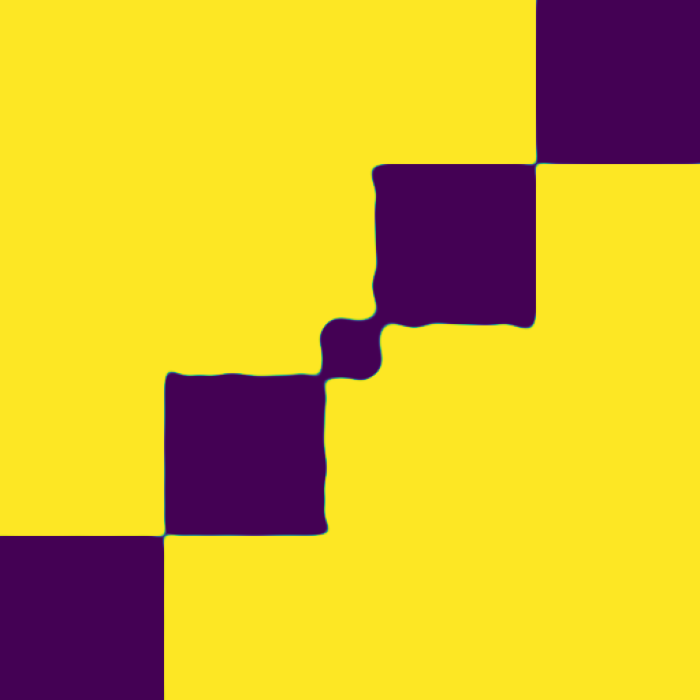
\includegraphics[width=4.2cm]{img/layer_6.png}};
  \draw[arr] (head.north) |- (img.west);
  \node[font=\small,anchor=south] at (27.7,12.15) {$W=f_\theta[c]$};
  % constraint solver
  \node[draw=ink,line width=0.8mm,fill=white,rounded corners=2mm,minimum height=3.1cm,
        inner xsep=7mm,font=\normalsize] (solve) at (20.3,1.15)
    {\textbf{solver:}\;\; $c$ such that\;\;
     $\frac{1}{|\mathcal{E}|}\sum_{\mathcal{E}} f_\theta[c]=p$};
  \draw[arr] (head.south |- solve.north) -- (head.south)
    node[midway,right=2mm,font=\normalsize] {$c$};
  \node[font=\small,anchor=west] at (-1.85,2.3) {top row: encodings $\sin(U^{(\ell)}\mathbf{x})$ of};
  \node[font=\small,anchor=west] at (-1.85,1.2) {$\mathbf{x}=(\min(x_1,x_2),\,\max(x_1,x_2))$,};
  \node[font=\small,anchor=west] at (-1.85,0.1) {so $W$ is symmetric};
\end{tikzpicture}

\gap{8mm}
\sub{{\color{accent}1}\;\; Multi-scale sinusoidal residual network}
Every layer re-injects a sinusoidal encoding of the input, at a frequency
scale $s(\ell)=2^{\ell-1}$ that doubles with depth:
\[
  g^{(\ell)} = g^{(\ell-1)} + \phi\bigl(V^{(\ell-1)}g^{(\ell-1)} + W^{(\ell)}\sin(U^{(\ell)}\mathbf{x}) + b^{(\ell)}\bigr).
\]
Early layers fix the coarse blocks; late layers sharpen the boundaries.

\vspace{4mm}
\hmap{4.85cm}{layer_1}{$\ell=1$}\hfill
\hmap{4.85cm}{layer_2}{$\ell=2$}\hfill
\hmap{4.85cm}{layer_3}{$\ell=3$}\hfill
\hmap{4.85cm}{layer_4}{$\ell=4$}\hfill
\hmap{4.85cm}{layer_5}{$\ell=5$}\hfill
\hmap{4.85cm}{layer_6}{$\ell=6$}

\vspace{1.5mm}
\src{Output layer applied to the hidden state after layer $\ell$ of one trained
network ($K_3$, $p=7/9$).}

\gap{8mm}
\sub{{\color{accent}2}\;\; Constraint solver inside the forward pass}
The bias $c$ is not learnt. Each step solves the empirical constraint by
clipped Newton iterations and differentiates through the solution implicitly:
\[
  \nabla_\theta c_\theta = -\sum_{\mathbf{y}\in\mathcal{E}} w_\theta(\mathbf{y})\,\nabla_\theta h_\theta(\mathbf{y}),
  \qquad
  w_\theta(\mathbf{y})\propto\sigma'\bigl(h_\theta(\mathbf{y})+c_\theta\bigr),
\]
with $h_\theta = V g^{(6)}$. The same construction enforces $t(H,W)=r^{e(H)}$ in (P2).

\gap{8mm}
\sub{{\color{accent}3}\;\; Cosine-annealing learning rate}
\hl{High rates find the coarse structure; low rates refine the details.}

\vspace{3mm}
% schematic schedule: five cosine cycles with warm restarts
\begin{minipage}[t]{15.4cm}\vspace{0pt}
  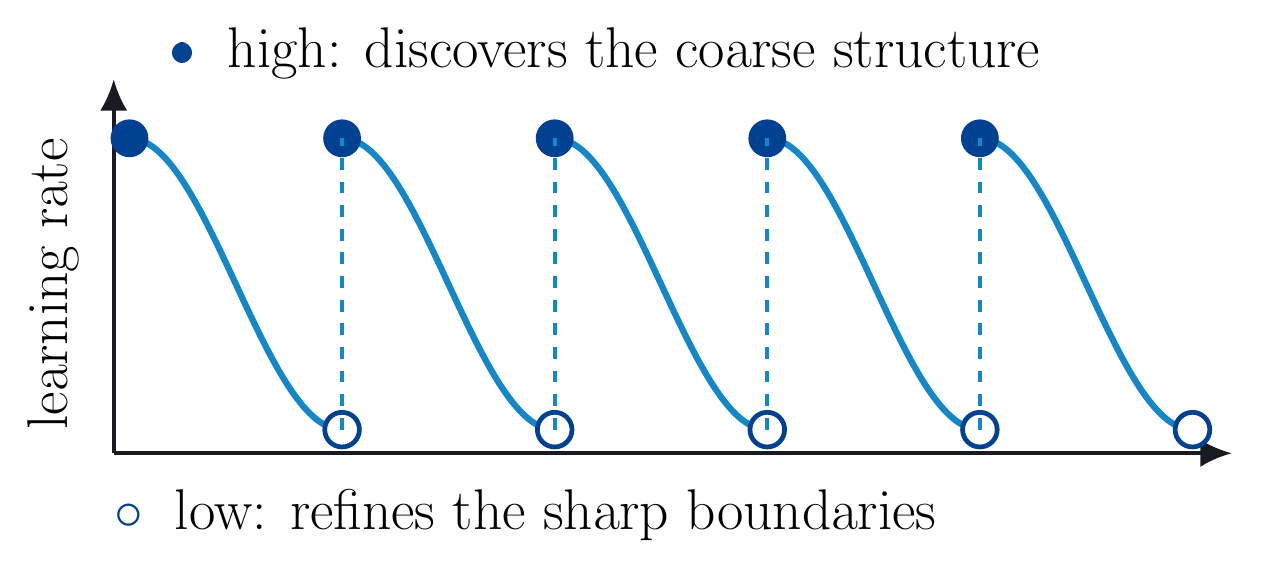
\begin{tikzpicture}[x=1cm,y=1cm]
    \draw[ink,line width=0.5mm,-{Latex[length=4mm,width=3.5mm]}] (1.1,0) -- (15.3,0);
    \draw[ink,line width=0.5mm,-{Latex[length=4mm,width=3.5mm]}] (1.1,0) -- (1.1,4.75);
    \node[font=\small,rotate=90,anchor=north,inner sep=0pt] at (0,2.15) {learning rate};
    \foreach \k in {0,...,4} {
      \draw[accent,line width=0.8mm,domain=0:2.7,samples=60,smooth,variable=\t]
        plot ({1.3+\k*2.7+\t},{0.3+3.7*(1+cos(180*\t/2.7))/2});
      \fill[main] (1.3+\k*2.7,4.0) circle[radius=2.4mm];
      \filldraw[fill=white,draw=main,line width=0.6mm] (4.0+\k*2.7,0.3) circle[radius=2.2mm];
    }
    \foreach \k in {1,...,4}
      \draw[accent,line width=0.5mm,dash pattern=on 1.5mm off 1.5mm] (1.3+\k*2.7,0.3) -- (1.3+\k*2.7,4.0);
    \node[font=\small,anchor=south west,inner sep=0pt] at (1.8,4.75)
      {{\color{main}\textbullet}\; high: discovers the coarse structure};
    \node[font=\small,anchor=north west,inner sep=0pt] at (1.1,-0.45)
      {{\color{main}$\circ$}\; low: refines the sharp boundaries};
  \end{tikzpicture}
\end{minipage}\hfill
\hmap{4.75cm}{abl_lr_low}{always low\\ 0.43754}\hfill
\hmap{4.75cm}{abl_lr_high}{always high\\ 0.43617}\hfill
\hmap{4.75cm}{abl_ours}{\textbf{cosine (ours)}\\ \textbf{0.43571}}

\gap{6mm}
\src{Training: Adam, width 256, depth 6, one RTX A5000; 30 min ($K_3$) to a few
hours (Petersen).}
\end{minipage}\end{lrbox}

% ======================================================================
% Column C -- results for (P1)
% ======================================================================
\newlength{\hw}\setlength{\hw}{6.4cm}
\begin{lrbox}{\colC}\begin{minipage}[t][\colheight][s]{46.4cm}\rr
\sectx{Results \textperiodcentered{} (P1)}{Extremal graph theory: known, open, new}{%
  learnt graphons on $[0,1]^2$:\;\; $W=0$\;
  \raisebox{-1.2mm}{
\includegraphics[width=8cm,height=7mm]{img/colorbar.png}}\; $W=1$%
  \qquad percentages: gap to the reference value}

\sub{Rediscovers classical optima without human input}
Triangle density at six edge densities $p$: within \hl{0.05\%} of the optimum
($0.00008$ at $p=\tfrac12$, where the optimum is $0$). At $p=1-1/k$ the network
finds the complete $k$-partite graphon $\Wk$. \src{[Razborov 2008]}

\vspace{4mm}
\hmap{\hw}{k3_50}{$K_3$,\; $p=\tfrac12$}\hfill
\hmap{\hw}{k3_67}{$p=\tfrac23$ \;\textperiodcentered\; $+0.05\%$}\hfill
\hmap{\hw}{k3_80}{$p=\tfrac45$ \;\textperiodcentered\; $+0.02\%$}\hfill
\hmap{\hw}{k3_57}{$p=\tfrac47$ \;\textperiodcentered\; $+0.01\%$}\hfill
\hmap{\hw}{k3_62}{$p=\tfrac58$ \;\textperiodcentered\; $+0.01\%$}\hfill
\hmap{\hw}{k3_71}{$p=\tfrac57$ \;\textperiodcentered\; $+0.02\%$}

\vspace{5mm}
\hmap{\hw}{k4_75}{$K_4$,\; $p=\tfrac34$}\hfill
\hmap{\hw}{k5_80}{$K_5$,\; $p=\tfrac45$}\hfill
\hmap{\hw}{k6_83}{$K_6$,\; $p=\tfrac56$}\hfill
\begin{minipage}[t]{23.2cm}\rr\vspace{0pt}
  \begin{tabular}{@{}l@{\hspace{10mm}}l@{\hspace{10mm}}l@{}}
    \toprule
    $K_k$ density, $p=1-\tfrac1k$ & optimum & ours (95\% CI) \\
    \midrule
    $k=4$ & 0.09375 & [0.09404, 0.09411] \\
    $k=5$ & 0.03840 & [0.03868, 0.03872] \\
    $k=6$ & 0.01543 & [0.01566, 0.01568] \\
    \bottomrule
  \end{tabular}

  \vspace{5mm}
  Larger cliques: more blocks and a noisier estimator, and the complete
  $k$-partite structure is still recovered. \src{[Reiher 2016]}
\end{minipage}

\gap{7mm}
\sub{Open problems: odd cycles $C_5$ and $C_7$}
$C_5$: within \hl{0.1\%} of the conjecture of Bennett et al., with a banded
structure away from $p=1-1/k$. $C_7$: no prior results; we state a conjecture
and match it within \hl{0.1\%}. Below: $p=\tfrac47,\tfrac58,\tfrac57$.

\vspace{4mm}
\hmap{\hw}{c5_57}{$C_5$,\, $\tfrac47$ \,\textperiodcentered\, $+0.06\%$}\hfill
\hmap{\hw}{c5_62}{$C_5$,\, $\tfrac58$ \,\textperiodcentered\, $+0.04\%$}\hfill
\hmap{\hw}{c5_71}{$C_5$,\, $\tfrac57$ \,\textperiodcentered\, $+0.03\%$}\hfill
\hmap{\hw}{c7_57}{$C_7$,\, $\tfrac47$ \,\textperiodcentered\, $+0.09\%$}\hfill
\hmap{\hw}{c7_62}{$C_7$,\, $\tfrac58$ \,\textperiodcentered\, $+0.05\%$}\hfill
\hmap{\hw}{c7_71}{$C_7$,\, $\tfrac57$ \,\textperiodcentered\, $+0.02\%$}

\gap{7mm}
\sub{All 117 small graphs: a previously unreported structure}
Every non-bipartite $H$ on at most 6 vertices, at 6 densities: \hl{702
instances}, \hl{72.6\%} within 1\% of the flag-algebra lower bound. For $H_6$
we find graphons below both the $k$-partite and the constant one; they appear
to depend on the \hl{circular distance}.

\vspace{4mm}
\begin{minipage}[t]{\hw}\centering
  \vspace{0pt}
  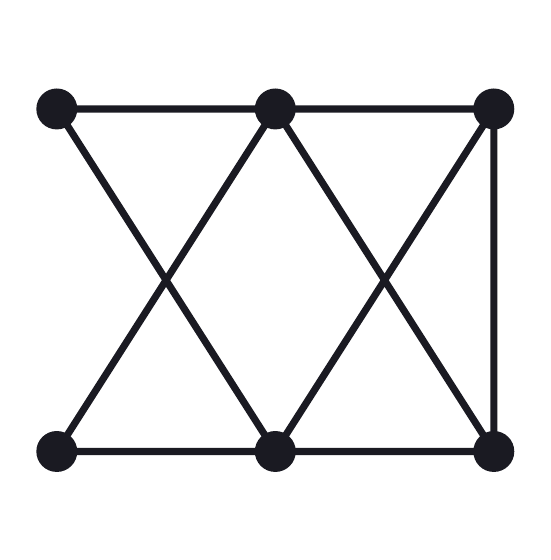
\begin{tikzpicture}[x=1.85cm,y=2.9cm]
    \foreach \n/\x/\y in {1/-1.5/1.5,2/-1.5/0,3/0/1.5,4/0/0,5/1.5/1.5,6/1.5/0}
      \coordinate (v\n) at (\x,\y);
    \draw[line width=0.9mm,color=ink]
      (v5)--(v4)--(v1)--(v3)--(v5)--(v6)--(v3)--(v2)--(v4)--(v6);
    \foreach \n in {1,...,6} \fill[ink] (v\n) circle[radius=2.6mm];
    \path (-1.7,-0.35) rectangle (1.7,1.856);
  \end{tikzpicture}\\[1.5mm]
  {\small the graph $H_6$\par}
\end{minipage}\hfill
\hmap{\hw}{h6_67}{$H_6$,\; $p=\tfrac23$}\hfill
\hmap{\hw}{h6_75}{$p=\tfrac34$}\hfill
\hmap{\hw}{h6_80}{$p=\tfrac45$}\hfill
\begin{minipage}[t]{15.4cm}\rr\vspace{0pt}
  \begin{tabular}{@{}c@{\hspace{6mm}}l@{\hspace{6mm}}l@{\hspace{6mm}}l@{}}
    \toprule
    $p$ & \textbf{ours} & $k$-partite & constant \\
    \midrule
    2/3 & \textbf{0.02476} & 0.03292 & 0.02601 \\
    3/4 & \textbf{0.07219} & 0.07617 & 0.07508 \\
    4/5 & \textbf{0.12986} & 0.13056 & 0.13422 \\
    \bottomrule
  \end{tabular}

  \vspace{2mm}
  \src{$t(H_6,W)$; lower is better.}
\end{minipage}\par\vspace{0pt}
\end{minipage}\end{lrbox}

% ======================================================================
% Column D -- results for (P2), ablation
% ======================================================================
\newlength{\dw}
\begin{lrbox}{\colD}\begin{minipage}[t][\colheight][s]{26cm}\rr
\sect{Results \textperiodcentered{} (P2)}{Large deviations of $G(n,q)$}

\sub{New candidate optima in both tails}
Upper tail ($q=0.1$, $r=0.5$): \hl{two-block} graphons for every pattern,
with similar blocks for the 2-regular $K_3$, $C_4$, $C_5$. Lower tail
($q=0.8$, $r=0.05$): nearly bipartite.

\vspace{4mm}
\setlength{\dw}{4.75cm}
\hmap{\dw}{ld_k3}{$K_3$}\hfill
\hmap{\dw}{ld_c4}{$C_4$}\hfill
\hmap{\dw}{ld_c5}{$C_5$}\hfill
\hmap{\dw}{ld_k13}{$K_{1,3}$}\hfill
\hmap{\dw}{ld_lower}{$K_3$, lower tail}

\gap{7mm}
\sub{Better than the best-known construction}
Relative entropy $h_q(W)$ for $H=K_3$, upper tail; lower is better.

\vspace{2mm}
\begin{tabular*}{\linewidth}{@{\extracolsep{\fill}}llll@{}}
  \toprule
  $(q,\,r)$ & Lubetzky--Zhao & \textbf{ours} & lower bound \\
  \midrule
  (0.05, 0.4) & 0.5561 & \textbf{0.4642} & 0.4603 \\
  (0.05, 0.5) & 0.8304 & \textbf{0.7279} & 0.7253 \\
  (0.05, 0.6) & 1.1449 & \textbf{1.0512} & 1.0492 \\
  (0.10, 0.4) & 0.3112 & \textbf{0.3091} & 0.3066 \\
  (0.10, 0.5) & 0.5108 & \textbf{0.5061} & 0.5043 \\
  (0.10, 0.6) & 0.7507 & \textbf{0.7477} & 0.7460 \\
  \bottomrule
\end{tabular*}

\vspace{3mm}
The tripartite construction of Lubetzky--Zhao (2015) is suboptimal in all six
regimes; ours is within 1\% of their lower bound.

\gap{5mm}
\sect{Ablation}{What matters}

$K_3$ at $p=7/9$; the optimum is $98/225\approx 0.43556$.

\vspace{4mm}
\setlength{\dw}{5.6cm}
\hmap{\dw}{abl_ours}{\textbf{ours}\\ \textbf{0.43571}}\hfill
\hmap{\dw}{abl_reg}{penalty term\\ 0.43709}\hfill
\hmap{\dw}{abl_sbm}{SBM, 256 blocks\\ 0.43582}\hfill
\hmap{\dw}{abl_tree}{decision tree\\ 0.45556}

\vspace{4mm}
\begin{itemize}
  \item A penalty instead of the solver, or a constant learning rate, gives a
        higher density.
  \item Encoding in the first layer only, or at one constant scale: similar
        density, often without sharp straight boundaries.
  \item Non-neural step-function baselines rarely leave the geometry of
        their initialisation.
\end{itemize}\par\vspace{0pt}
\end{minipage}\end{lrbox}

% ======================================================================
% Theorems
% ======================================================================
\newcommand{\thmcard}[3]{% title, body, source
  \begin{minipage}[t]{31.6cm}\rr
    {\large\bfseries\color{main}#1\par}\vspace{3mm}
    #2\par\vspace{3mm}
    \src{#3}
  \end{minipage}}

\begin{lrbox}{\thmIntro}\begin{minipage}[t]{25.2cm}\rr
  {\small\bfseries\color{accent}\MakeUppercase{From pictures to proofs}\par}\vspace{1.5mm}
  {\Large\bfseries\color{main}Three new theorems\par}\vspace{5mm}
  The graphons found by our method motivated three theorems: two on the
  complete $k$-partite structure, one on the two-block structure.

  \vspace{5mm}
  \src{$\Wk$: the balanced complete $k$-partite graphon.}
\end{minipage}\end{lrbox}

\begin{lrbox}{\thmA}\thmcard{Odd cycles}{%
  Let $m\ge 3$ be odd and $t(K_2,W)=p\ge 2/3$. Then
  \[ t(C_m,W)\;\ge\;p^m-p\,(1-p)^{m-1}. \]
  Hence $\Wk$ minimises the density of \emph{every} odd cycle at $p=1-1/k$, for
  all $k\ge 3$: the structure learnt for $C_7$ at $p=\tfrac23,\tfrac45$ is optimal.}{%
  Im, Kim, Yang (2026), arXiv:2610.18277}\end{lrbox}

\begin{lrbox}{\thmB}\thmcard{Chordal graphs}{%
  Let $H$ be a connected chordal graph whose maximal cliques all have the same
  size $r\ge 3$. Then, for every integer $k\ge r$,
  \[ \Wk\ \text{ minimises }\ t(H,W)\ \text{ subject to }\ t(K_2,W)=1-\tfrac1k. \]
  This settles 48 instances of our sweep, for 16 graphs other than cliques.}{%
  This paper; proof formalised in Lean~4: github.com/mekty2012/PureChordalGoodman}\end{lrbox}

\begin{lrbox}{\thmC}\thmcard{Bipodal upper tails}{%
  Let $H$ be $d$-regular, $d\ge 2$, and $r\ne\tfrac{d-1}{d}$. Close to the
  boundary $q_c(r)$ of the region where the constant graphon is optimal, for
  $q<q_c(r)$, the minimiser of $h_q(W)$ subject to $t(H,W)\ge r^{e(H)}$ is
  \emph{unique}, nonconstant and \emph{bipodal}: constant on $A\times A$,
  $A\times B$ and $B\times B$ for a partition $[0,1]=A\cup B$.}{%
  Lim, Im, Kim, Nam, Yang (2026), arXiv:2609.15222, Theorem~1.5}\end{lrbox}

\report{column A (background)}{\colA}
\report{column B (method)}{\colB}
\report{column C (P1)}{\colC}
\report{column D (P2)}{\colD}
\report{theorem intro}{\thmIntro}
\report{theorem A}{\thmA}
\report{theorem B}{\thmB}
\report{theorem C}{\thmC}

% ======================================================================
% Page
% ======================================================================
\begin{tikzpicture}[remember picture,overlay,shift={(current page.north west)},x=1cm,y=1cm]
  \fill[paper] (0,0) rectangle (140,-90);

  % ---- header band
  \fill[main] (0,0) rectangle (140,-13.3);
  \node[anchor=north west,inner sep=0pt] at (2.5,-1.7) {\parbox{90cm}{\rr
    {\fontsize{92pt}{101pt}\selectfont\bfseries\color{white}
      Implicit Neural Representations\\ for Variational Problems on Graphons\par}
    \vspace{7mm}
    {\fontsize{42pt}{50pt}\selectfont\color{white}
      \textbf{Taeyoung Kim}\textsuperscript{1,2}\qquad Jineon Baek\textsuperscript{3}\qquad
      Joonkyung Lee\textsuperscript{2}\qquad Hongseok Yang\textsuperscript{1,2}\par}
    \vspace{3mm}
    {\fontsize{26pt}{32pt}\selectfont\color{white!82!main}
      \textsuperscript{1}School of Computing, KAIST\qquad
      \textsuperscript{2}School of Computational Sciences, KIAS\qquad
      \textsuperscript{3}June E Huh Center for Mathematical Challenges, KIAS\qquad
      taeyoungkim21@kaist.ac.kr\par}}};

  % institution logos: the white variants from the KAIST and KIAS brand kits
  \node[anchor=west,inner sep=0pt] at (61.6,-6.65)
    {
\includegraphics[height=3.7cm]{img/logos/kaist_white.png}};
  \node[anchor=west,inner sep=0pt] at (77.0,-6.65)
    {
\includegraphics[height=6.6cm]{img/logos/kias_white.png}};

  % one-sentence takeaway
  \node[anchor=west,inner sep=0pt] at (94.2,-6.65) {\parbox{24cm}{\rr
    {\fontsize{34pt}{44pt}\selectfont\color{white}
      Gradient descent on a neural graphon\\
      rediscovers classical extremal graphs,\\
      proposes candidates for open problems,\\
      and has led to new theorems.\par}}};

  % links, side by side: the NeurIPS poster page and the code
  \node[anchor=north east,fill=white,inner sep=4.5mm] (qrcode) at (137.5,-1.5)
    {\qrcode[height=7cm]{https://github.com/mekty2012/INR4GraphonVariationalProblem}};
  \node[anchor=north east,fill=white,inner sep=4.5mm] (qrpaper) at ($(qrcode.north west)+(-1.0,0)$)
    {\qrcode[height=7cm]{https://nips.cc/virtual/2026/loc/sydney/poster/153602}};
  \node[anchor=north,align=center,inner sep=0pt,color=white] at ($(qrpaper.south)+(0,-0.35)$)
    {{\fontsize{26pt}{31pt}\selectfont\bfseries Paper}\\
     {\fontsize{19pt}{24pt}\selectfont\color{white!82!main} NeurIPS 2026 page}};
  \node[anchor=north,align=center,inner sep=0pt,color=white] at ($(qrcode.south)+(0,-0.35)$)
    {{\fontsize{26pt}{31pt}\selectfont\bfseries Code}\\
     {\fontsize{19pt}{24pt}\selectfont\color{white!82!main} GitHub}};

  % ---- columns
  \node[anchor=north west,inner sep=0pt] at (2.5,-15.0)   {\usebox{\colA}};
  \node[anchor=north west,inner sep=0pt] at (29.5,-15.0)  {\usebox{\colB}};
  \node[anchor=north west,inner sep=0pt] at (63.3,-15.0)  {\usebox{\colC}};
  \node[anchor=north west,inner sep=0pt] at (111.5,-15.0) {\usebox{\colD}};

  % ---- theorem band
  \fill[tint] (0,-75.8) rectangle (140,-90);
  \fill[accent] (0,-75.8) rectangle (140,-76.15);
  \node[anchor=north west,inner sep=0pt] at (2.5,-77.2) {\usebox{\thmIntro}};
  \foreach \b/\x in {\thmA/29.5,\thmB/66.1,\thmC/102.7} {
    \fill[white] (\x,-77.1) rectangle ++(34.8,-10.0);
    \node[anchor=north west,inner sep=0pt] at (\x+1.6,-77.95) {\usebox{\b}};
  }

  % ---- acknowledgement
  \node[anchor=north west,inner sep=0pt] at (2.5,-87.5) {\parbox{135cm}{\rr
    \fontsize{17.5pt}{22.5pt}\selectfont\color{muted}
    \textbf{Acknowledgements.} T.~Kim and H.~Yang were
    supported by the National Research Foundation of Korea (NRF) grant funded by the
    Korean Government (MSIT) (No.~RS-2023-00279680).
    H.~Yang was also supported by a KIAS Individual Grant (CG109601) at the Korea
    Institute for Advanced Study.\\
    J.~Lee was supported by Samsung STF Grant
    (SSTF-BA2201-02) and the NRF grant funded by the Korean Government (MSIT)
    (No.~NRF-2022R1C1C1010300). J.~Baek was supported by KIAS Individual Grant
    (HP105001).}};
\end{tikzpicture}
\end{document}
